\documentclass[11pt,letterpaper]{article}
\PassOptionsToPackage{hyphens}{url}
\usepackage[margin=.83in,top=.8in,bottom=.8in,headheight=15pt]{geometry}
\usepackage[T1]{fontenc}
\usepackage{lmodern,amsmath,amssymb,mathtools,bm,booktabs,array,graphicx,tikz}
\usetikzlibrary{arrows.meta,positioning,calc,decorations.pathreplacing,patterns}
\definecolor{ink}{HTML}{17344D}\definecolor{accent}{HTML}{087E8B}\definecolor{pale}{HTML}{EDF5F5}\definecolor{gold}{HTML}{AD6B19}
\providecommand{\dd}{\,\mathrm{d}}\providecommand{\R}{\mathbb{R}}
\providecommand{\E}{\mathbb{E}}\providecommand{\Var}{\operatorname{Var}}
\providecommand{\Cov}{\operatorname{Cov}}\providecommand{\diag}{\operatorname{diag}}
\providecommand{\norm}[1]{\left\lVert#1\right\rVert}
\providecommand{\abs}[1]{\left|#1\right|}
\usepackage{microtype,hyperref,fancyhdr,enumitem,amsthm,sectsty,needspace}
\allsectionsfont{\raggedright}
\hypersetup{colorlinks=true,linkcolor=ink,urlcolor=accent,pdfauthor={Zan Ahmad},pdftitle={Finite-volume advection and diffusion / Lecture notes}}
\setlength{\parindent}{0pt}\setlength{\parskip}{6pt}\linespread{1.07}
\setlist{itemsep=3pt,topsep=4pt,leftmargin=*}
\emergencystretch=2em\clubpenalty=10000\widowpenalty=10000
\pagestyle{fancy}\fancyhf{}\fancyhead[L]{\small Computational Cardiology}\fancyhead[R]{\small Lecture 5}
\fancyfoot[L]{\footnotesize Zan Ahmad}\fancyfoot[R]{\footnotesize\thepage}\renewcommand{\headrulewidth}{.3pt}
\newtheorem{proposition}{Proposition}\newtheorem{theorem}{Theorem}\newtheorem{lemma}{Lemma}
\theoremstyle{definition}\newtheorem{definition}{Definition}\newtheorem{example}{Example}
\numberwithin{equation}{section}
\begin{document}
{\small\scshape Computational Cardiology\hfill Lecture 5}\par\medskip
{\raggedright\hyphenpenalty=10000\exhyphenpenalty=10000\LARGE\bfseries\color{ink} Finite-volume advection and diffusion\par}\medskip
{\small Lecture notes}\par\bigskip
A spatial conservation law is a collection of local balances joined by shared interface fluxes. For advection--diffusion, this construction exposes both the global boundary budget and the time-step restriction required for a nonnegative explicit update.

\section{Control volumes and the boundary budget}
\hypertarget{note-control-volumes-and-the-boundary-budget}{}\label{note:control-volumes-and-the-boundary-budget}
{\small \href{slides.html\#frame=the-represented-concentration\&step=1}{Slides for this section} \quad \href{../modules/cfd/index.html}{Conservation, viscous flow and transport} \quad \href{../modules/animations/conservation-flow.html}{Conservation and channel flow}}\par
A compartment balance already says that stored amount changes by inflow minus outflow. A spatial model applies that idea to many adjacent control volumes. Divide a straight one-dimensional domain into equal cells of width \ensuremath{\Delta}x and unit cross-sectional area. Store each cell's average concentration c, rather than its value at an arbitrarily chosen point. In this synthetic lesson concentration is dimensionless, so amount per unit area has units of meters. If concentration were mass per volume, the same balance would instead track mass per area.

Let J at a face denote rightward flux. The left face contributes positively to the cell; the right face contributes negatively. Multiplying the difference by the time step gives the change in cell amount. Neighboring cells must use exactly the same numerical face flux with opposite signs. This shared value is what makes internal transfers cancel. Computing two slightly different fluxes on the two sides of one face would break the account even if both formulas looked plausible.

Summing all cells leaves only the two boundary faces. On a periodic domain the first and last faces represent the same interface and their flux values agree, so total amount is constant. On an open domain the total may change, but only by the integrated boundary input minus output. A nonconstant total is therefore not automatically a numerical failure. The relevant test is agreement with the correct boundary budget.

\[
\Delta x\,(c_i^{n+1}-c_i^n)=\Delta t\,(J_{i-1/2}^n-J_{i+1/2}^n)
\]
J is positive to the right; for dimensionless concentration J has m/s.

\[
M^{n+1}-M^n=\Delta t\,(J_{1/2}^n-J_{N+1/2}^n),\quad M=\Delta x\sum_i c_i
\]
All internal face contributions cancel exactly in real arithmetic.

Define the represented state by an integral, rather than by a point sample:
\[
 \bar c_i(t)=\frac1{\Delta x}\int_{x_{i-1/2}}^{x_{i+1/2}}c(x,t)\,\mathrm dx.
\]
Integrating $c_t+J_x=0$ over the cell gives $\Delta x\,\dot{\bar c}_i=J_{i-1/2}-J_{i+1/2}$. Summation telescopes because each interior face belongs to two adjacent cells with opposite signs.
\section{Advective and diffusive fluxes}
\hypertarget{note-advective-and-diffusive-fluxes}{}\label{note:advective-and-diffusive-fluxes}
{\small \href{slides.html\#frame=constitutive-transport-flux-figure\&step=1}{Slides for this section} \quad \href{../modules/cfd/index.html}{Conservation, viscous flow and transport} \quad \href{../modules/animations/conservation-flow.html}{Conservation and channel flow}}\par
For a prescribed velocity a, advection carries concentration with the moving medium. Its continuum flux is a times c. Diffusion represents net spreading down a concentration gradient, so its flux is minus D times the spatial slope. A positive slope gives a negative diffusive flux: material moves to the left toward smaller concentration. D is nonnegative and has units of square meters per second. Both flux terms consequently have the same units and can be added.

The local differential equation follows by dividing the cell balance by width and letting width and time step become small. The flux derivative becomes a spatial derivative. With constant a and D, the concentration time derivative equals minus a times its first spatial derivative plus D times its second spatial derivative. This derivative statement describes the limiting model. Our implementation keeps the finite-volume balance because it makes the discrete accounting explicit.

Advection and diffusion are different mechanisms even when a plot shows both moving and smoothing. Pure continuum advection shifts a profile without changing its shape on this periodic domain. Diffusion spreads it and reduces peaks. Our upwind numerical approximation can also smooth a profile even when D is zero. Thus a rounded pulse alone cannot identify physical diffusion. Later refinement will distinguish numerical spreading from the specified diffusion coefficient.

\[
J=ac-D\,\partial_x c,\qquad \partial_t c+\partial_xJ=0
\]
a has m/s, D has m\ensuremath{^{2}}/s; c is dimensionless.

\[
\partial_t c=-a\partial_xc+D\partial_{xx}c
\]
The sign of the diffusion term follows from the minus sign in its flux.

For either sign of the velocity, write $a^+=\max(a,0)$ and $a^-=\min(a,0)$. A single numerical face flux is
\[
 J_{i+1/2}=a^+c_i+a^-c_{i+1}-D\frac{c_{i+1}-c_i}{\Delta x}.
\]
The upwind choice uses the concentration transported toward the interface. The diffusion term uses a centered difference and has the opposite sign to the concentration gradient.
\begin{center}\begin{minipage}{.98\linewidth}\centering
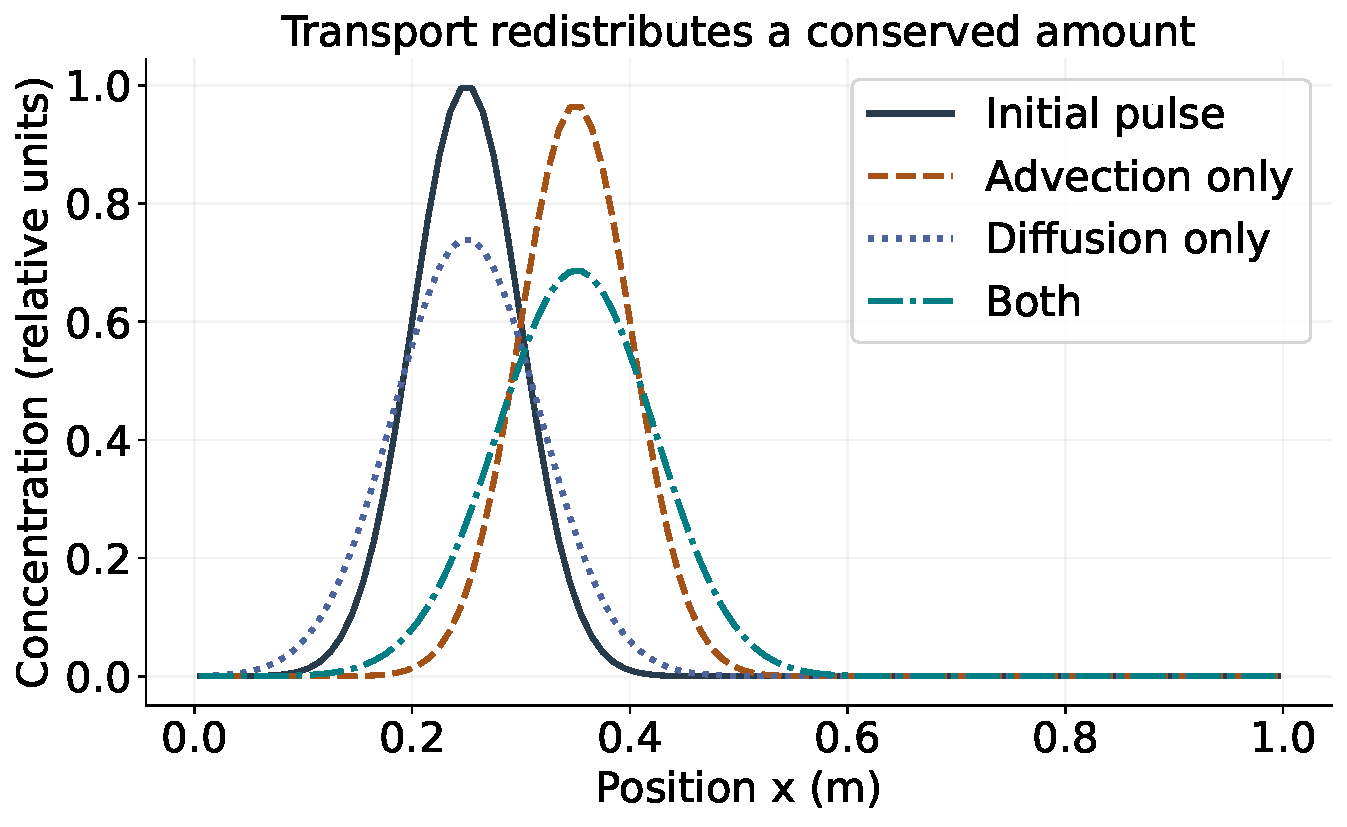
\includegraphics[width=.96\linewidth,height=.57\textheight,keepaspectratio]{transport-pulse.pdf}\par\smallskip
{\small Original periodic transport calculations at 0.5 s on 100 cells. Upwind advection also produces numerical spreading; plotted broadening is not all physical diffusion.}
\end{minipage}\end{center}
\section{The upwind stencil and a discrete maximum principle}
\hypertarget{note-the-upwind-stencil-and-a-discrete-maximum-principle}{}\label{note:the-upwind-stencil-and-a-discrete-maximum-principle}
{\small \href{slides.html\#frame=upwind-advection\&step=1}{Slides for this section} \quad \href{../modules/cfd/index.html}{Conservation, viscous flow and transport} \quad \href{../modules/animations/conservation-flow.html}{Conservation and channel flow}}\par
For positive velocity the upstream concentration at a face is in the cell immediately to its left. For negative velocity it is in the cell to its right. This is the first-order upwind choice. The centered diffusive face slope is the difference of neighboring cell concentrations divided by their center spacing. First compute every shared face flux; then update every cell from the old state. Updating cells in place would mix old and new values and implement another method.

For positive a, collecting coefficients in the update produces three weights: \ensuremath{\nu}+\ensuremath{\mu} on the left neighbor, 1\ensuremath{-}\ensuremath{\nu}\ensuremath{-}2\ensuremath{\mu} on the cell itself, and \ensuremath{\mu} on the right neighbor. Here \ensuremath{\nu}=a\ensuremath{\Delta}t/\ensuremath{\Delta}x and \ensuremath{\mu}=D\ensuremath{\Delta}t/\ensuremath{\Delta}x\ensuremath{^{2}}. They sum to one. If all are nonnegative, every new concentration lies between the smallest and largest of these old values. This convex-combination argument explains both nonnegativity and a simple maximum bound without invoking a general stability theorem.

For either velocity sign, the sufficient restriction is |a|\ensuremath{\Delta}t/\ensuremath{\Delta}x+2D\ensuremath{\Delta}t/\ensuremath{\Delta}x\ensuremath{^{2}}\ensuremath{\le}1. The supplied solver rejects a requested step that exceeds it and shortens the accepted step to land exactly at the requested endpoint. Halving cell width doubles the advective rate and quadruples the diffusive rate. Keeping the old time step after mesh refinement can therefore break the condition even though the spatial formula has not changed.

\[
c_i^{n+1}=(\nu+\mu)c_{i-1}^n+(1-\nu-2\mu)c_i^n+\mu c_{i+1}^n
\]
\ensuremath{\nu}=a\ensuremath{\Delta}t/\ensuremath{\Delta}x and \ensuremath{\mu}=D\ensuremath{\Delta}t/\ensuremath{\Delta}x\ensuremath{^{2}}; reverse the upwind neighbor for negative a.

\[
|a|\Delta t/\Delta x+2D\Delta t/\Delta x^2\le1
\]
This is a sufficient positivity condition for this explicit stencil, not a universal CFD criterion.

Set $\nu_+=a^+\Delta t/\Delta x$, $\nu_-=-a^-\Delta t/\Delta x$ and $\mu=D\Delta t/\Delta x^2$. The general stencil is
\[
 c_i^{n+1}=(\nu_++\mu)c_{i-1}^n+
 (1-\nu_+-\nu_--2\mu)c_i^n+(\nu_-+\mu)c_{i+1}^n.
\]
The coefficients sum to one. Their nonnegativity implies preservation of any interval containing the old values. This is a local maximum principle, stronger than conservation alone.
\section{An open-boundary calculation}
\hypertarget{note-an-open-boundary-calculation}{}\label{note:an-open-boundary-calculation}
{\small \href{slides.html\#frame=an-open-boundary-step-panel-1\&step=1}{Slides for this section} \quad \href{../modules/cfd/index.html}{Conservation, viscous flow and transport}}\par
Consider three cells, each 0.5 m wide, with concentrations 1, 2 and 1. During a 0.2 s step the four rightward face fluxes are prescribed as 0.3, 0.5, 0.2 and 0.1 m/s. These face values are a budget illustration, not values recomputed from a particular velocity and diffusion coefficient. Working with imposed fluxes first separates the accounting law from the constitutive formula used to generate those fluxes.

The first cell loses 0.04 m of amount per unit area, because its output exceeds its input by 0.2 m/s for 0.2 s. The second gains 0.06 m and the third gains 0.02 m. Dividing those changes by 0.5 m gives concentration changes \ensuremath{-}0.08, 0.12 and 0.04. The new concentrations are therefore 0.92, 2.12 and 1.04. Their total amount is 2.04 m, compared with an initial 2 m.

The net external input is 0.2 times (0.3\ensuremath{-}0.1), or 0.04 m. It matches the total change. Internal face fluxes 0.5 and 0.2 affect where the amount goes but disappear from the total budget. In the notebook, implement the difference of adjacent fluxes using this case, then test a changed internal face. The total should remain unchanged by that internal modification even though two neighboring concentrations change.

For the supplied four face fluxes,
\[
 \Delta c=\frac{0.2}{0.5}
 \begin{pmatrix}.3-.5\\.5-.2\\.2-.1\end{pmatrix}
 =\begin{pmatrix}-.08\\.12\\.04\end{pmatrix}.
\]
Changing the middle face by $\delta J$ adds $-\Delta t\,\delta J$ to one cell amount and $+\Delta t\,\delta J$ to its neighbor. The total budget is unaffected.

\paragraph{Calculation.} Compute all three concentrations and verify the net boundary account.

Apply c\_new=c\_old+(0.2/0.5)\ensuremath{\times}(left flux\ensuremath{-}right flux) to each cell.

Obtain 0.92, 2.12 and 1.04; multiply their sum by 0.5 m.

Compare 2.04\ensuremath{-}2=0.04 m with 0.2\ensuremath{\times}(0.3\ensuremath{-}0.1)=0.04 m.

The local updates and global open-boundary budget agree.
\begin{center}\begin{minipage}{.98\linewidth}\centering
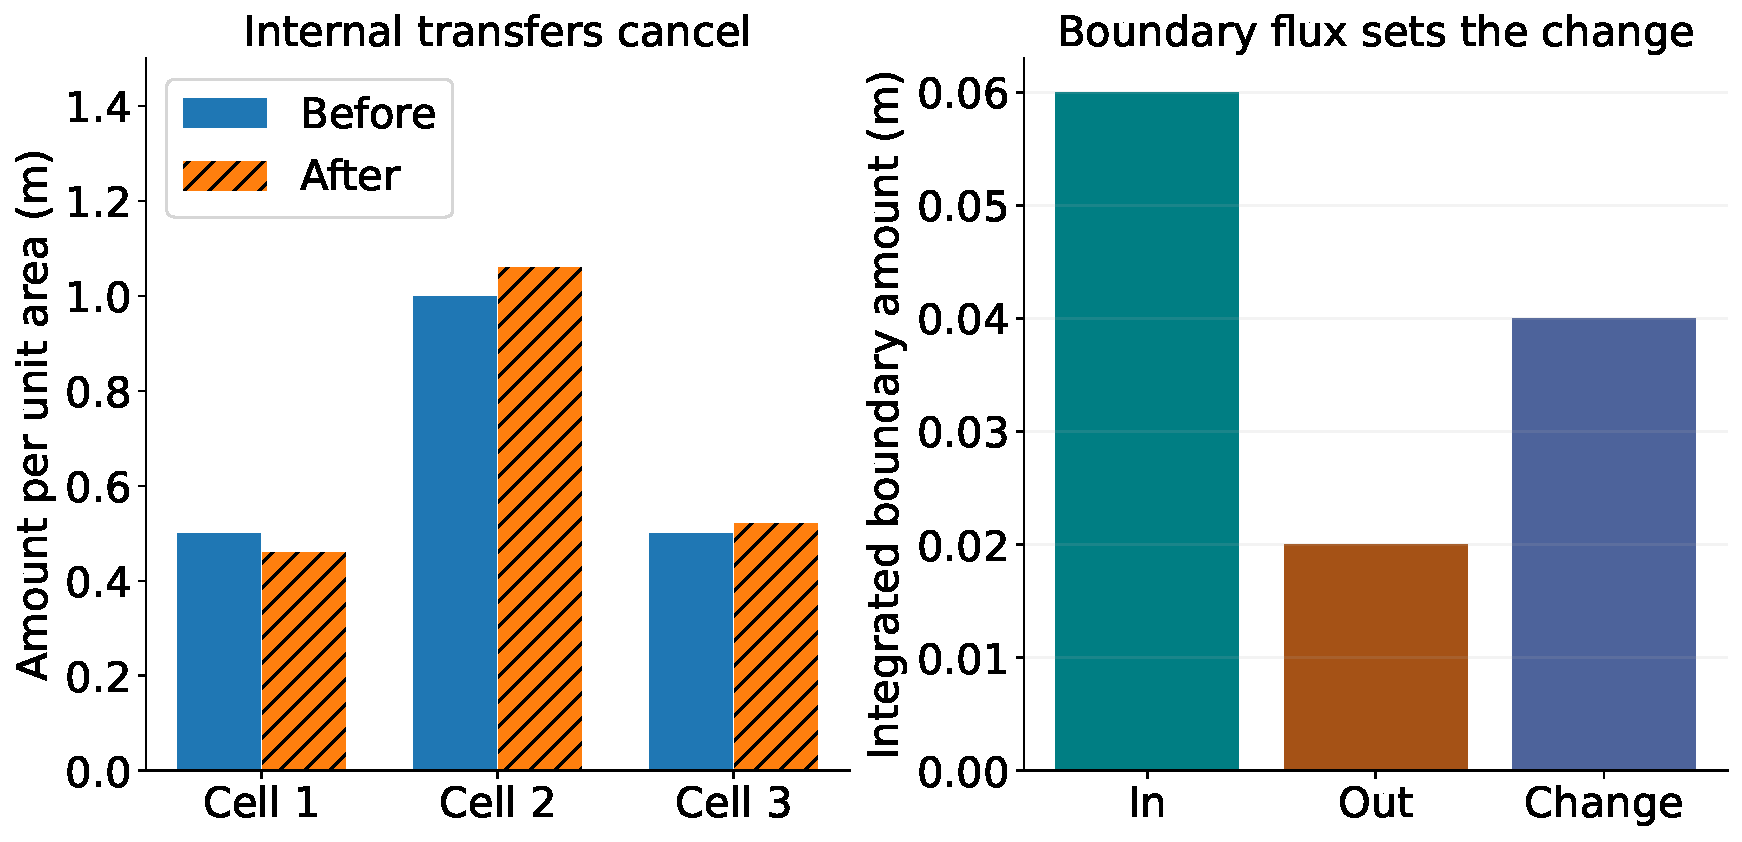
\includegraphics[width=.96\linewidth,height=.57\textheight,keepaspectratio]{flux-budget.pdf}\par\smallskip
{\small The worked three-cell example shows internal redistribution and a net boundary gain of 0.04 m of amount per unit area.}
\end{minipage}\end{center}
\section{Periodic transport and limiting cases}
\hypertarget{note-periodic-transport-and-limiting-cases}{}\label{note:periodic-transport-and-limiting-cases}
{\small \href{slides.html\#frame=an-exact-shift-of-the-cell-vector\&step=1}{Slides for this section} \quad \href{../modules/cfd/index.html}{Conservation, viscous flow and transport}}\par
The original demo starts a smooth pulse near x=0.25 m on a one-meter periodic domain and runs for 0.5 s with 100 cells. Three cases isolate positive advection, diffusion, and both together. A velocity of 0.2 m/s predicts a 0.1 m displacement of the continuum profile over this interval. The separate cases isolate each contribution to transport.

Before looking at the plot, record the predicted direction, broadening and total amount. After running, compare the initial and final discrete sums and inspect the minimum concentration. Test a constant state, for which every diffusive face flux vanishes and advective inflow equals outflow. Test zero velocity and zero diffusion, for which the entire state should remain identical. At unit advection number and zero diffusion, the upwind method shifts the cell vector exactly one cell; testing both velocity signs catches a frequent indexing error.

These checks answer different questions. Conservation alone would not reveal a reversed advection direction, and a constant-state test would not measure pulse smearing. A nonnegative but badly smeared solution can still be inaccurate. Numerical parameters and actual step size determine the amount of numerical smoothing. Concentration plots and integral diagnostics should be read together.

For pure positive advection with $\nu=1$, the update reduces to $c_i^{n+1}=c_{i-1}^n$, an exact one-cell shift of the represented vector. For $a=D=0$, the update is the identity. For constant $c_i$, all shared-flux differences vanish even when the individual advective fluxes are nonzero.
\Needspace{10\baselineskip}

\section{Physical and numerical diffusion}
\hypertarget{note-physical-and-numerical-diffusion}{}\label{note:physical-and-numerical-diffusion}
{\small \href{slides.html\#frame=numerical-diffusion\&step=1}{Slides for this section} \quad \href{../modules/cfd/index.html}{Conservation, viscous flow and transport}}\par
The same conservation structure will support more elaborate spatial models, but changing the application requires changing the modeled physics and boundaries. A tracer in a vessel would need a justified velocity field, geometry and inlet concentration. An electrical activation model also has local reaction terms and different state variables. The scalar pulse in this lesson cannot be reinterpreted as either application merely by relabeling its axes.

For positive advection, Taylor expansion of the fully discrete upwind scheme gives the leading modified equation
\[
 c_t+a c_x=\frac{a\Delta x}{2}(1-\nu)c_{xx}+\cdots
\]
when physical diffusion is absent and the solution is smooth. The added coefficient is numerical diffusion. It vanishes at the exact-shift case $\nu=1$ and decreases with mesh spacing at fixed $\nu$. A broadened numerical pulse therefore does not, by itself, measure a physical diffusivity.
\bigskip
\section*{Exercises}
\par\noindent\begin{minipage}{\linewidth}
\subsection*{E1. A four-cell boundary budget}
Use four cells of width 0.25 m, initial concentrations [1,2,3,2], a step of 0.1 s, and rightward face fluxes [0.4,0.2,0.5,0.3,0.1] m/s.

\textbf{a} Compute the new concentration in every cell.

\end{minipage}\par\medskip
\textbf{b} Verify the change in total amount against the boundaries.

\textbf{c} Increase only the middle face flux from 0.5 to 0.7. What changes in the total?

\par\noindent\begin{minipage}{\linewidth}
\subsection*{E2. Choose a safe explicit step}
Let a=\allowbreak{}0.15 m/s, D=\allowbreak{}0.001 m$^2$/s and $\Delta$x=\allowbreak{}0.02 m.

\textbf{a} Find the maximum step from the sufficient positivity condition.

\end{minipage}\par\medskip
\textbf{b} Halve $\Delta$x and recompute the bound. Explain the scaling.

\textbf{c} Does meeting this bound prove that the pulse shape is accurate?

\par\noindent\begin{minipage}{\linewidth}
\subsection*{E3. Design a diagnostic suite}
A periodic solver preserves total amount but transports a pulse left when a is positive.

\textbf{a} Name a check that exposes the error without relying on visual judgment.

\end{minipage}\par\medskip
\textbf{b} Explain why the total and constant-state tests both miss it.

\textbf{c} Propose a test for accidental double counting of an internal face.

\section*{References}
\noindent\begin{minipage}{\linewidth}
Zan Ahmad, Advanced Topics in Computational Cardiology syllabus, Fall 2024. PDF pages 1--2.

\end{minipage}\par\medskip
\noindent\begin{minipage}{\linewidth}
Hoppensteadt and Peskin, Modeling and Simulation in Medicine and the Life Sciences, second edition. Printed pages 313--315; supplied PDF pages 323--325 (random-walk conservation and diffusion bridge).

\end{minipage}\par\medskip
\end{document}
